% !TeX spellcheck = en_GB
\begin{figure}[H]
	\centering
	%%%%%% 20/12
	\begin{subfigure}[b]{0.49\textwidth}
		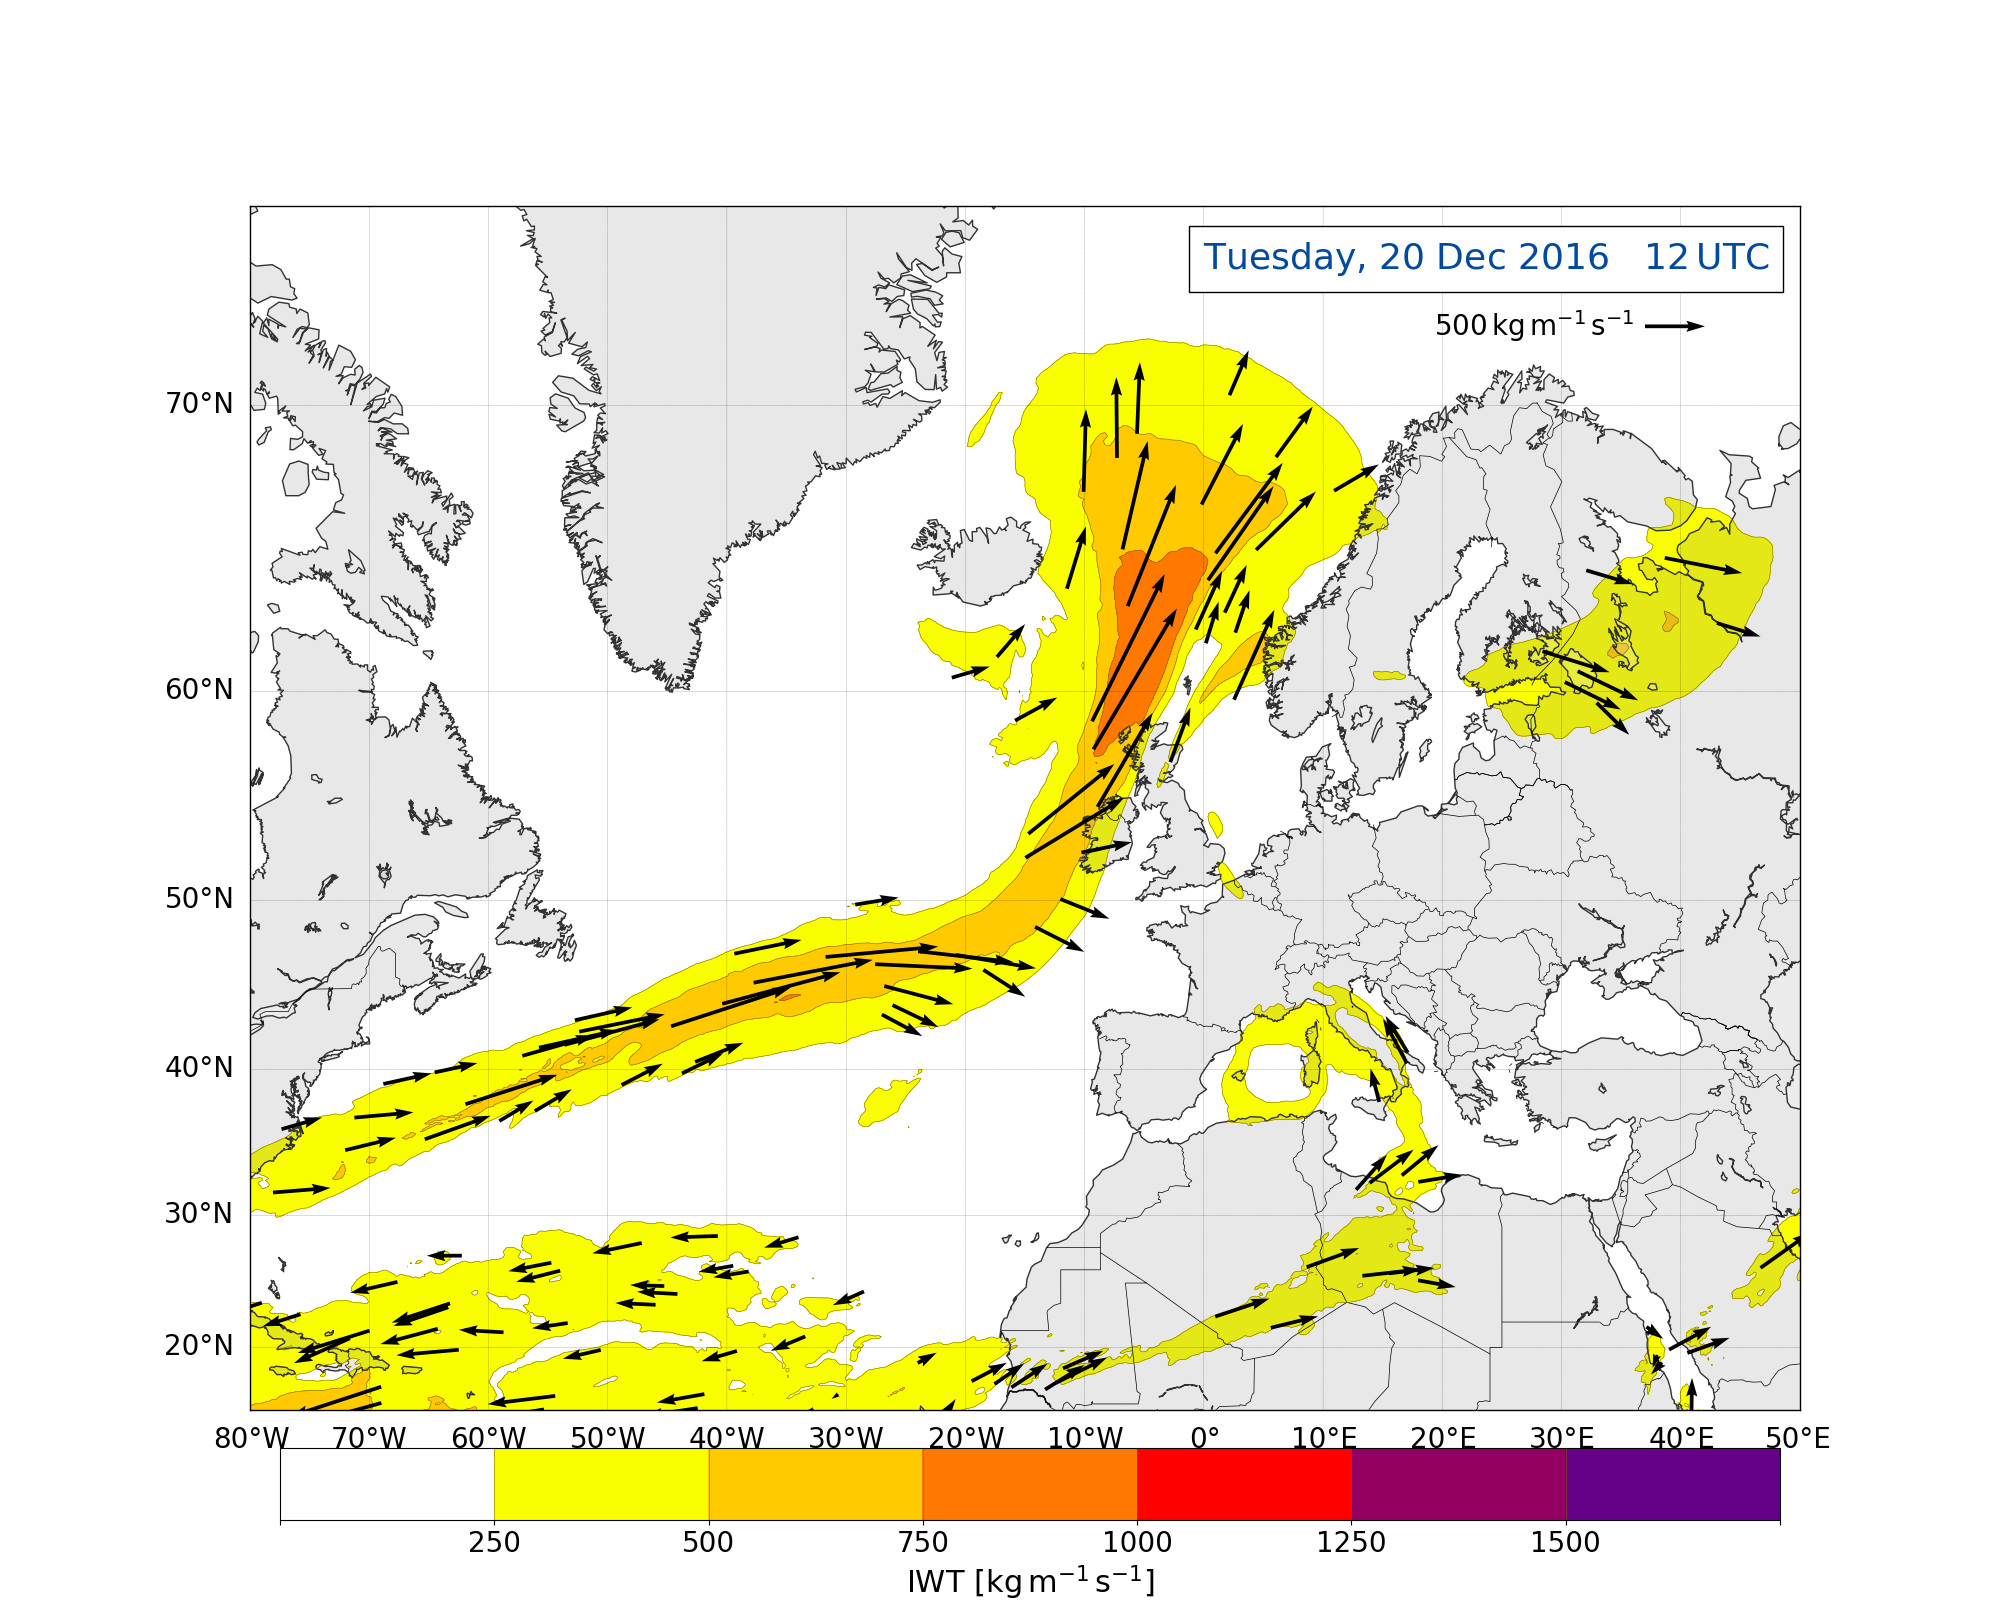
\includegraphics[trim={4.2cm 3.9cm 4.3cm 5.1cm},clip,
		width=\textwidth]{./fig_Atm_Riv/20161220_12}
		\caption{}\label{fig:AR20}
	\end{subfigure}
	%%%%%% 21/12
	\begin{subfigure}[b]{0.49\textwidth}
		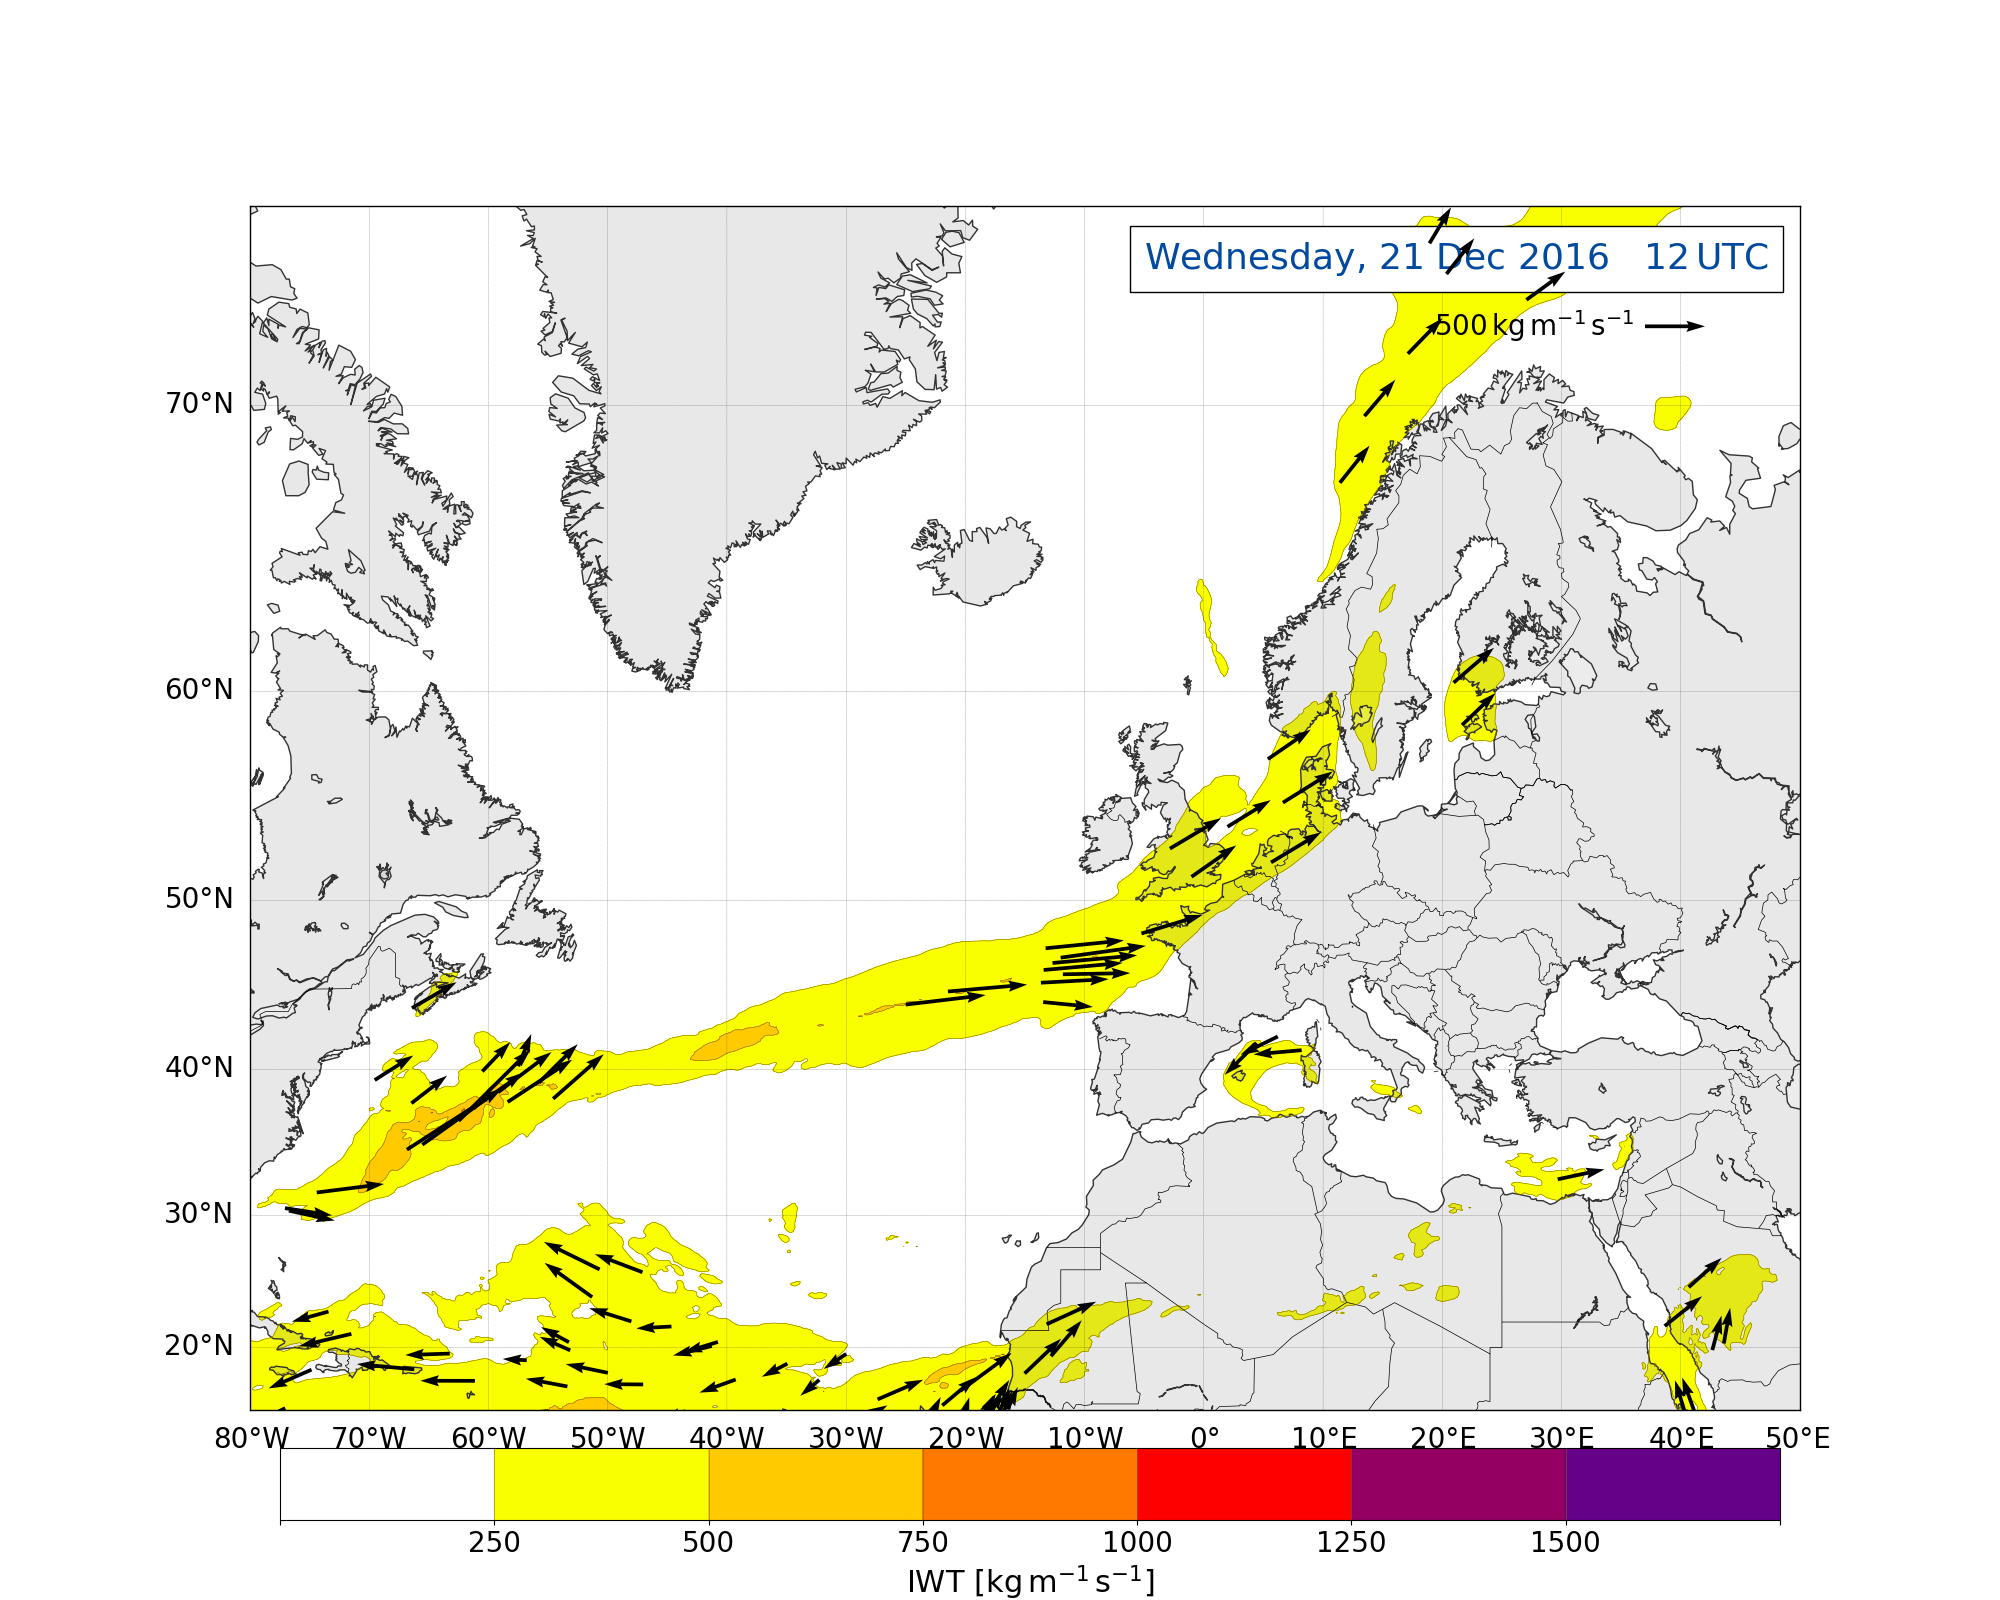
\includegraphics[trim={4.2cm 3.9cm 4.3cm 5.1cm},clip,
		width=\textwidth]{./fig_Atm_Riv/20161221_12}
		\caption{}\label{fig:AR21}
	\end{subfigure}
	%%%%%% label
	\begin{subfigure}[b]{\textwidth}
		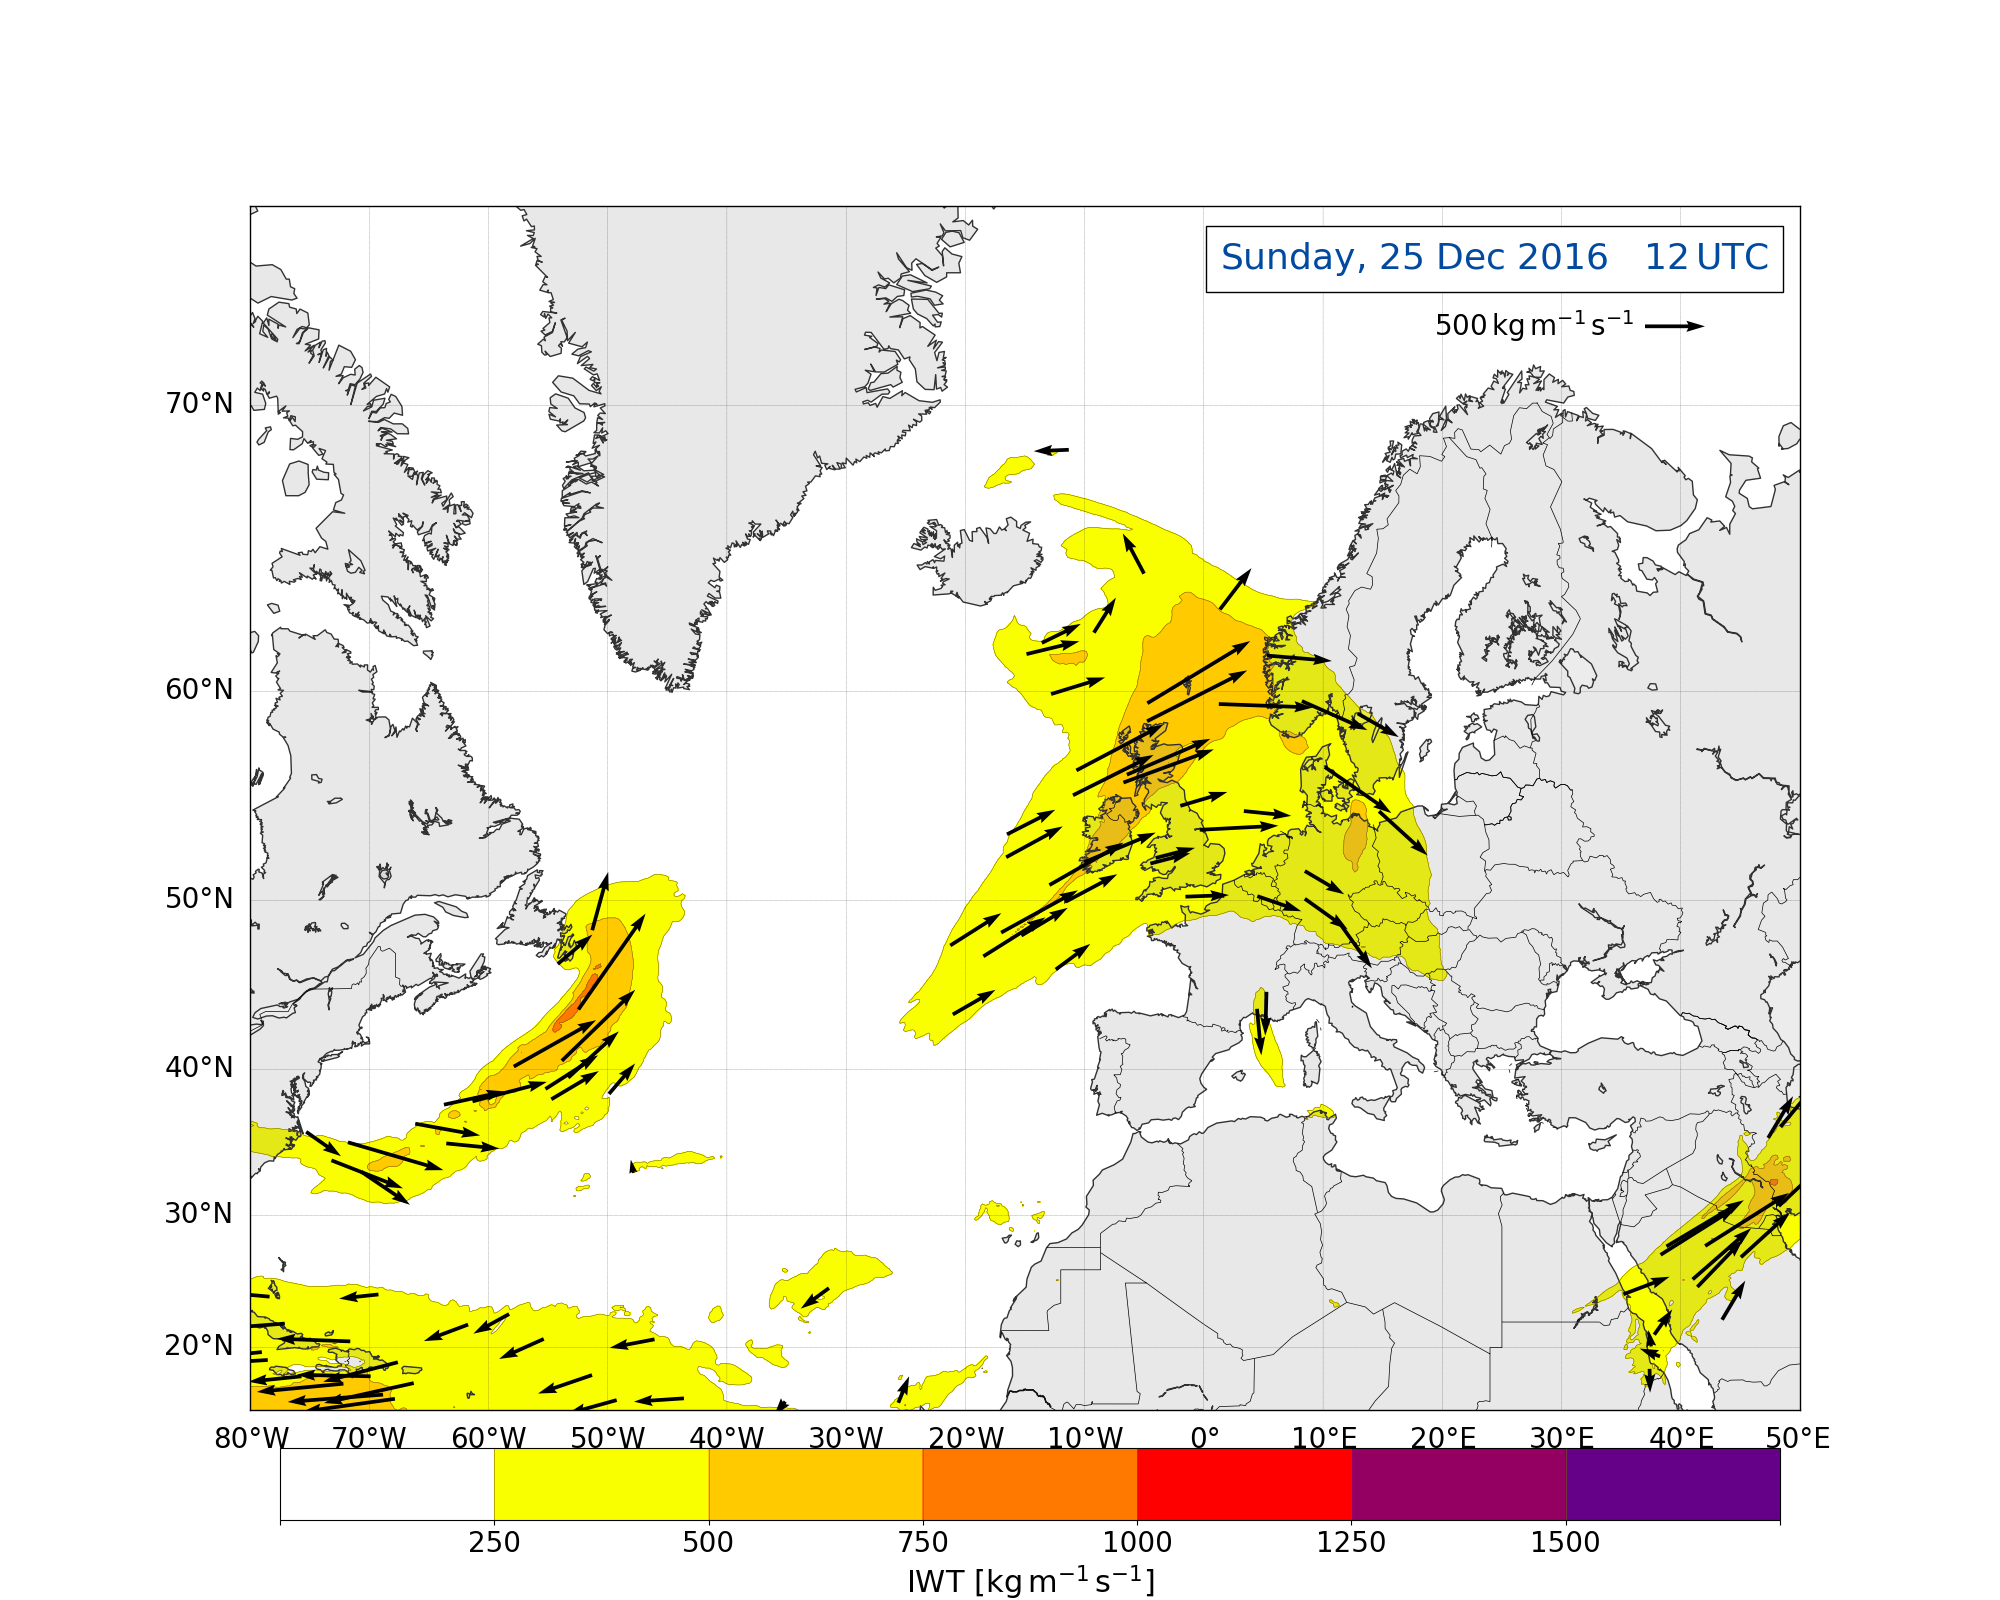
\includegraphics[trim={4.2cm 0cm 4.3cm 36.8cm},clip,
		width=\textwidth]{./fig_Atm_Riv/20161225_12}
	\end{subfigure}
\caption{Atmospheric river analysis map, data from ECMWF. During \SIrange{20}{27}{\dec}. IVT, shaded according to the colour bar [\SI{}{\IVT}]. Vectors, indicating the direction and magnitude of the IVT. }\label{fig:AtmRiv}
\end{figure}
%
\begin{figure}\ContinuedFloat
	\centering
	%%%%%% 22/12
	\begin{subfigure}[b]{0.49\textwidth}
		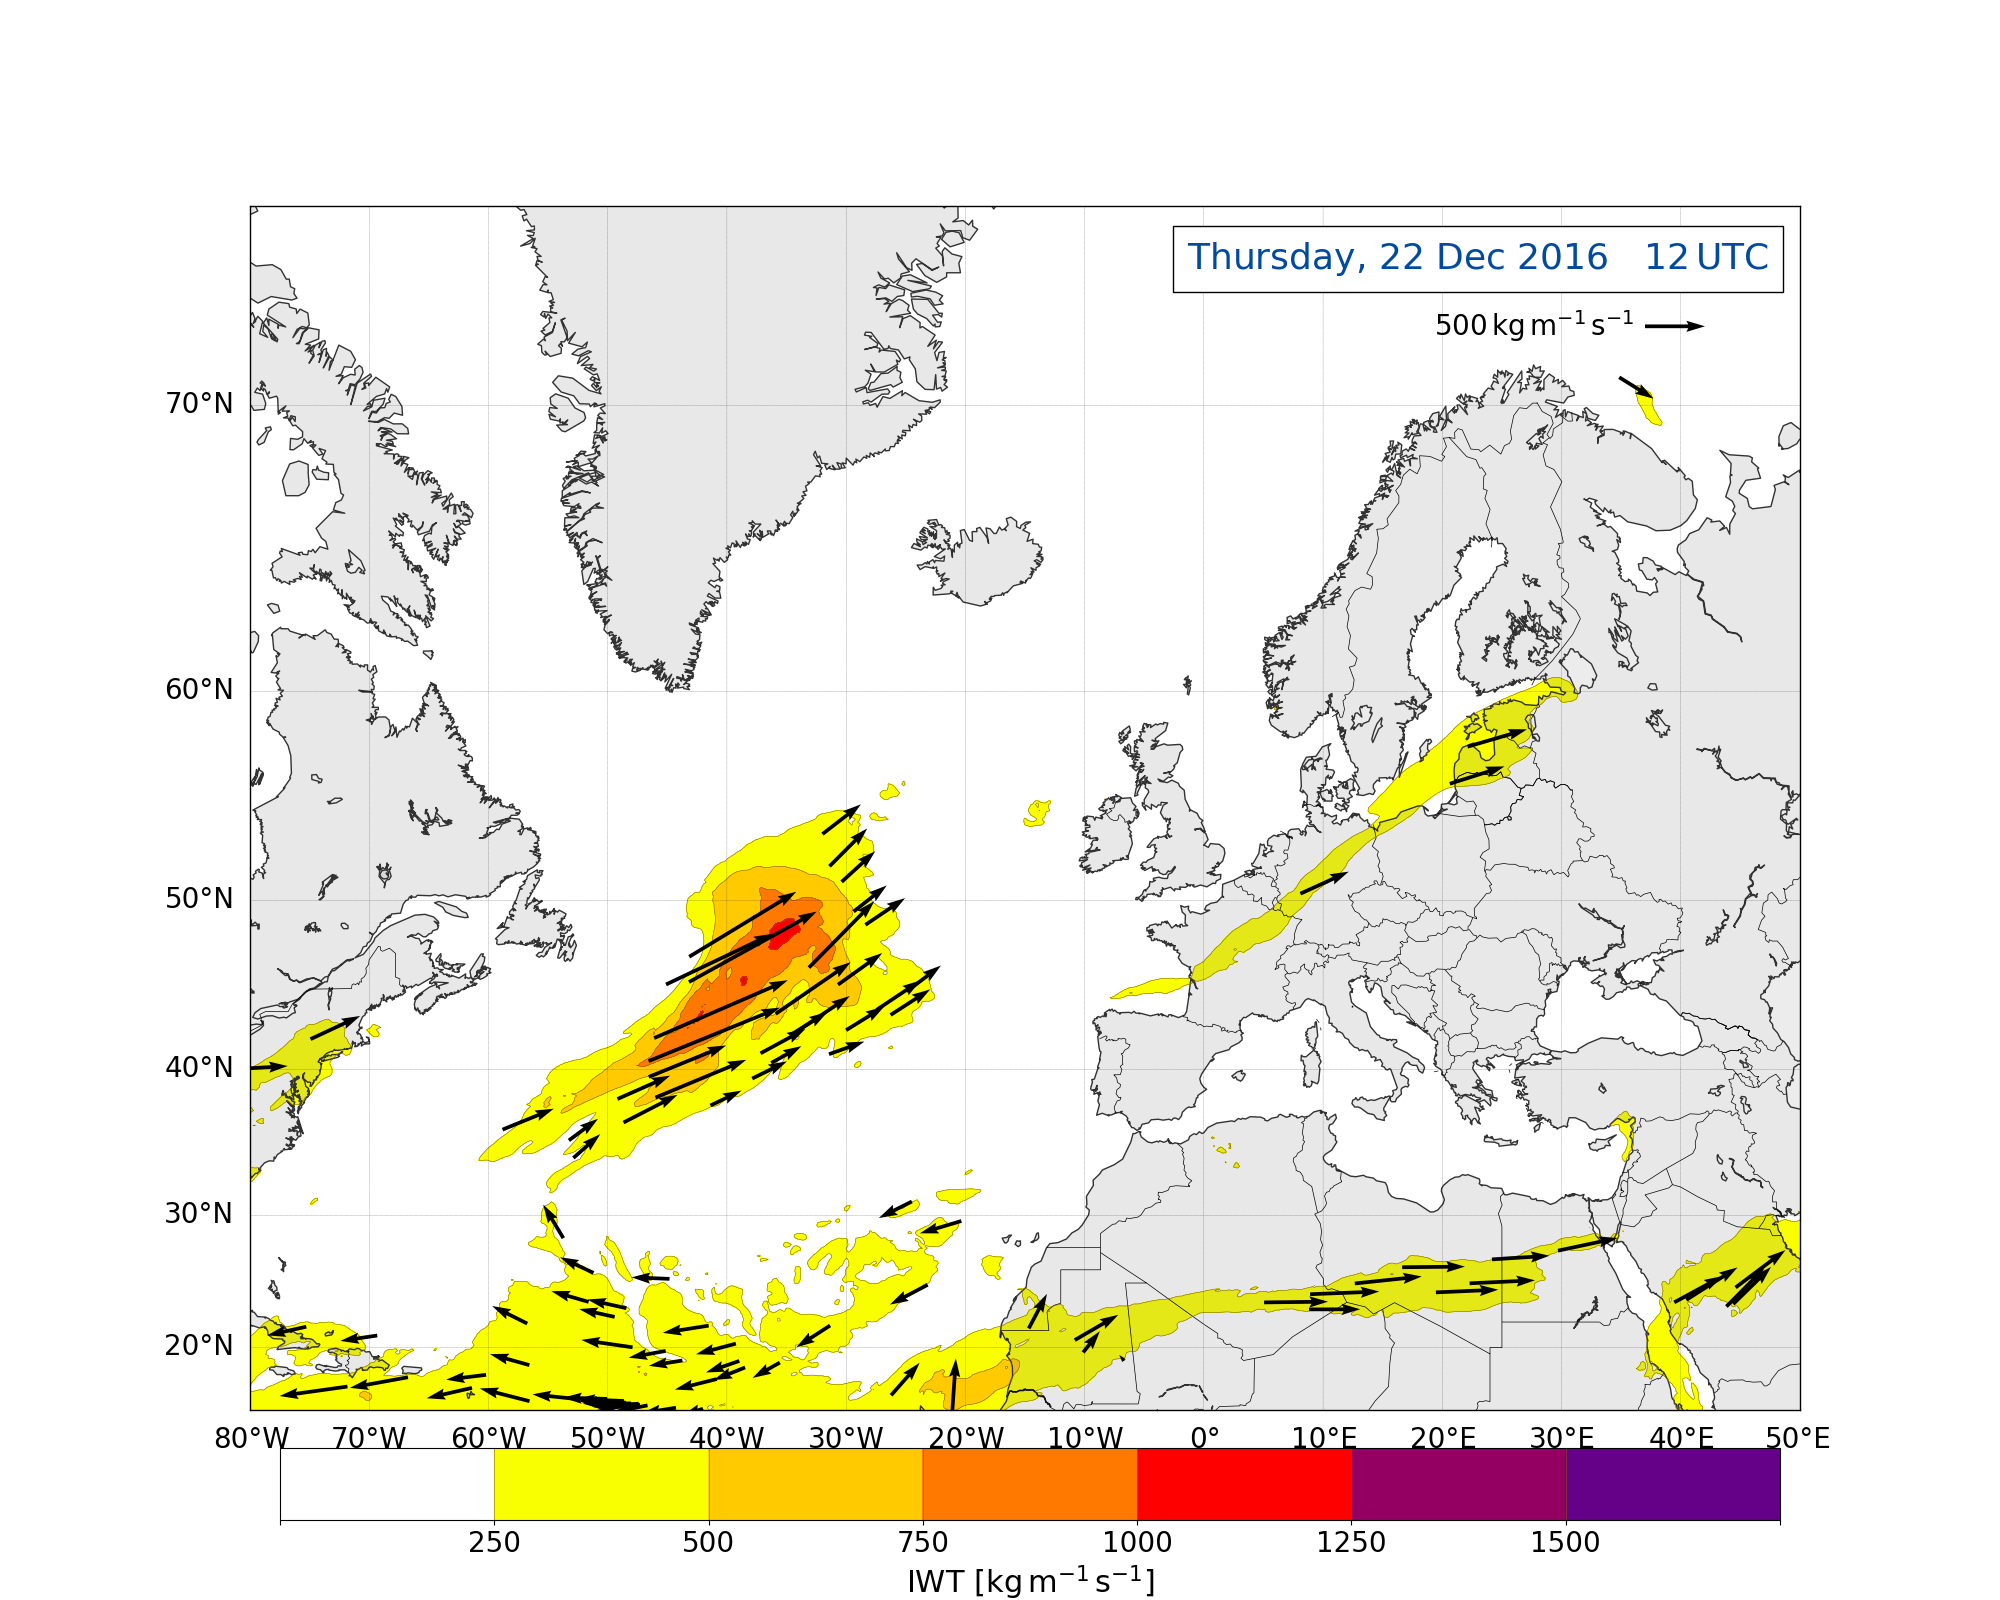
\includegraphics[trim={4.2cm 3.9cm 4.3cm 5.1cm},clip,
		width=\textwidth]{./fig_Atm_Riv/20161222_12}
		\caption{}\label{fig:AR22}
		%\label{fig:sfc2100}
	\end{subfigure}
	%%%%%% 23/12
	\begin{subfigure}[b]{0.49\textwidth}
		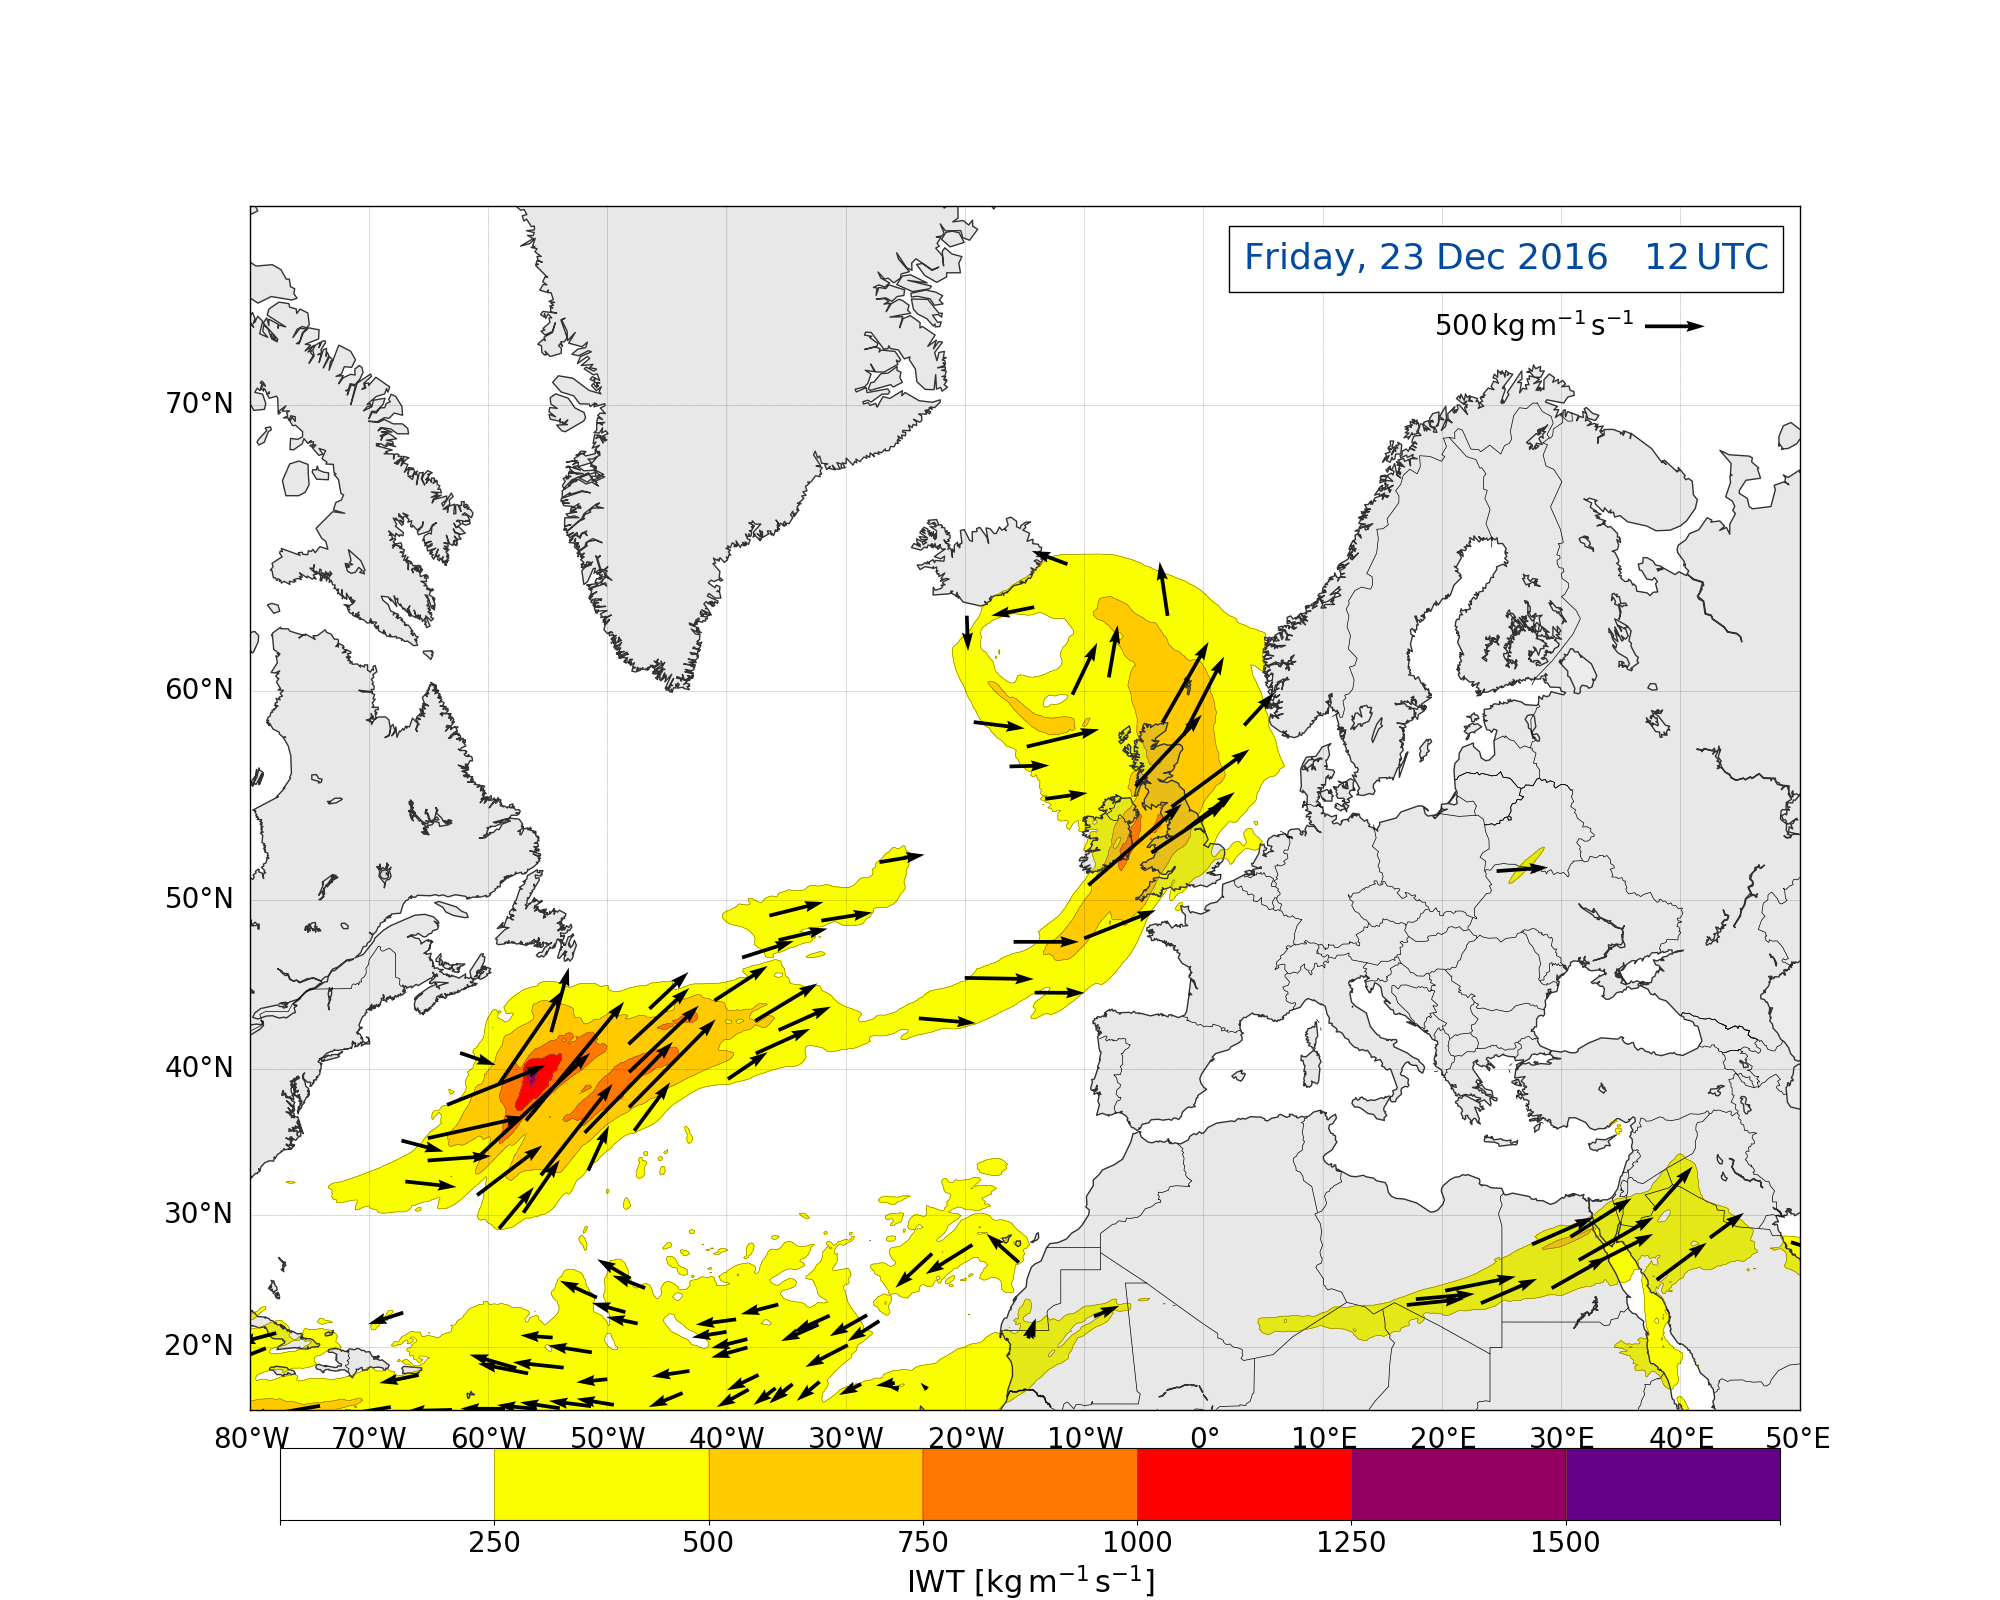
\includegraphics[trim={4.2cm 3.9cm 4.3cm 5.1cm},clip,
		width=\textwidth]{./fig_Atm_Riv/20161223_12}
		\caption{}\label{fig:AR23}
	\end{subfigure}
	%%%%%% 24/12
	\begin{subfigure}[b]{0.49\textwidth}
		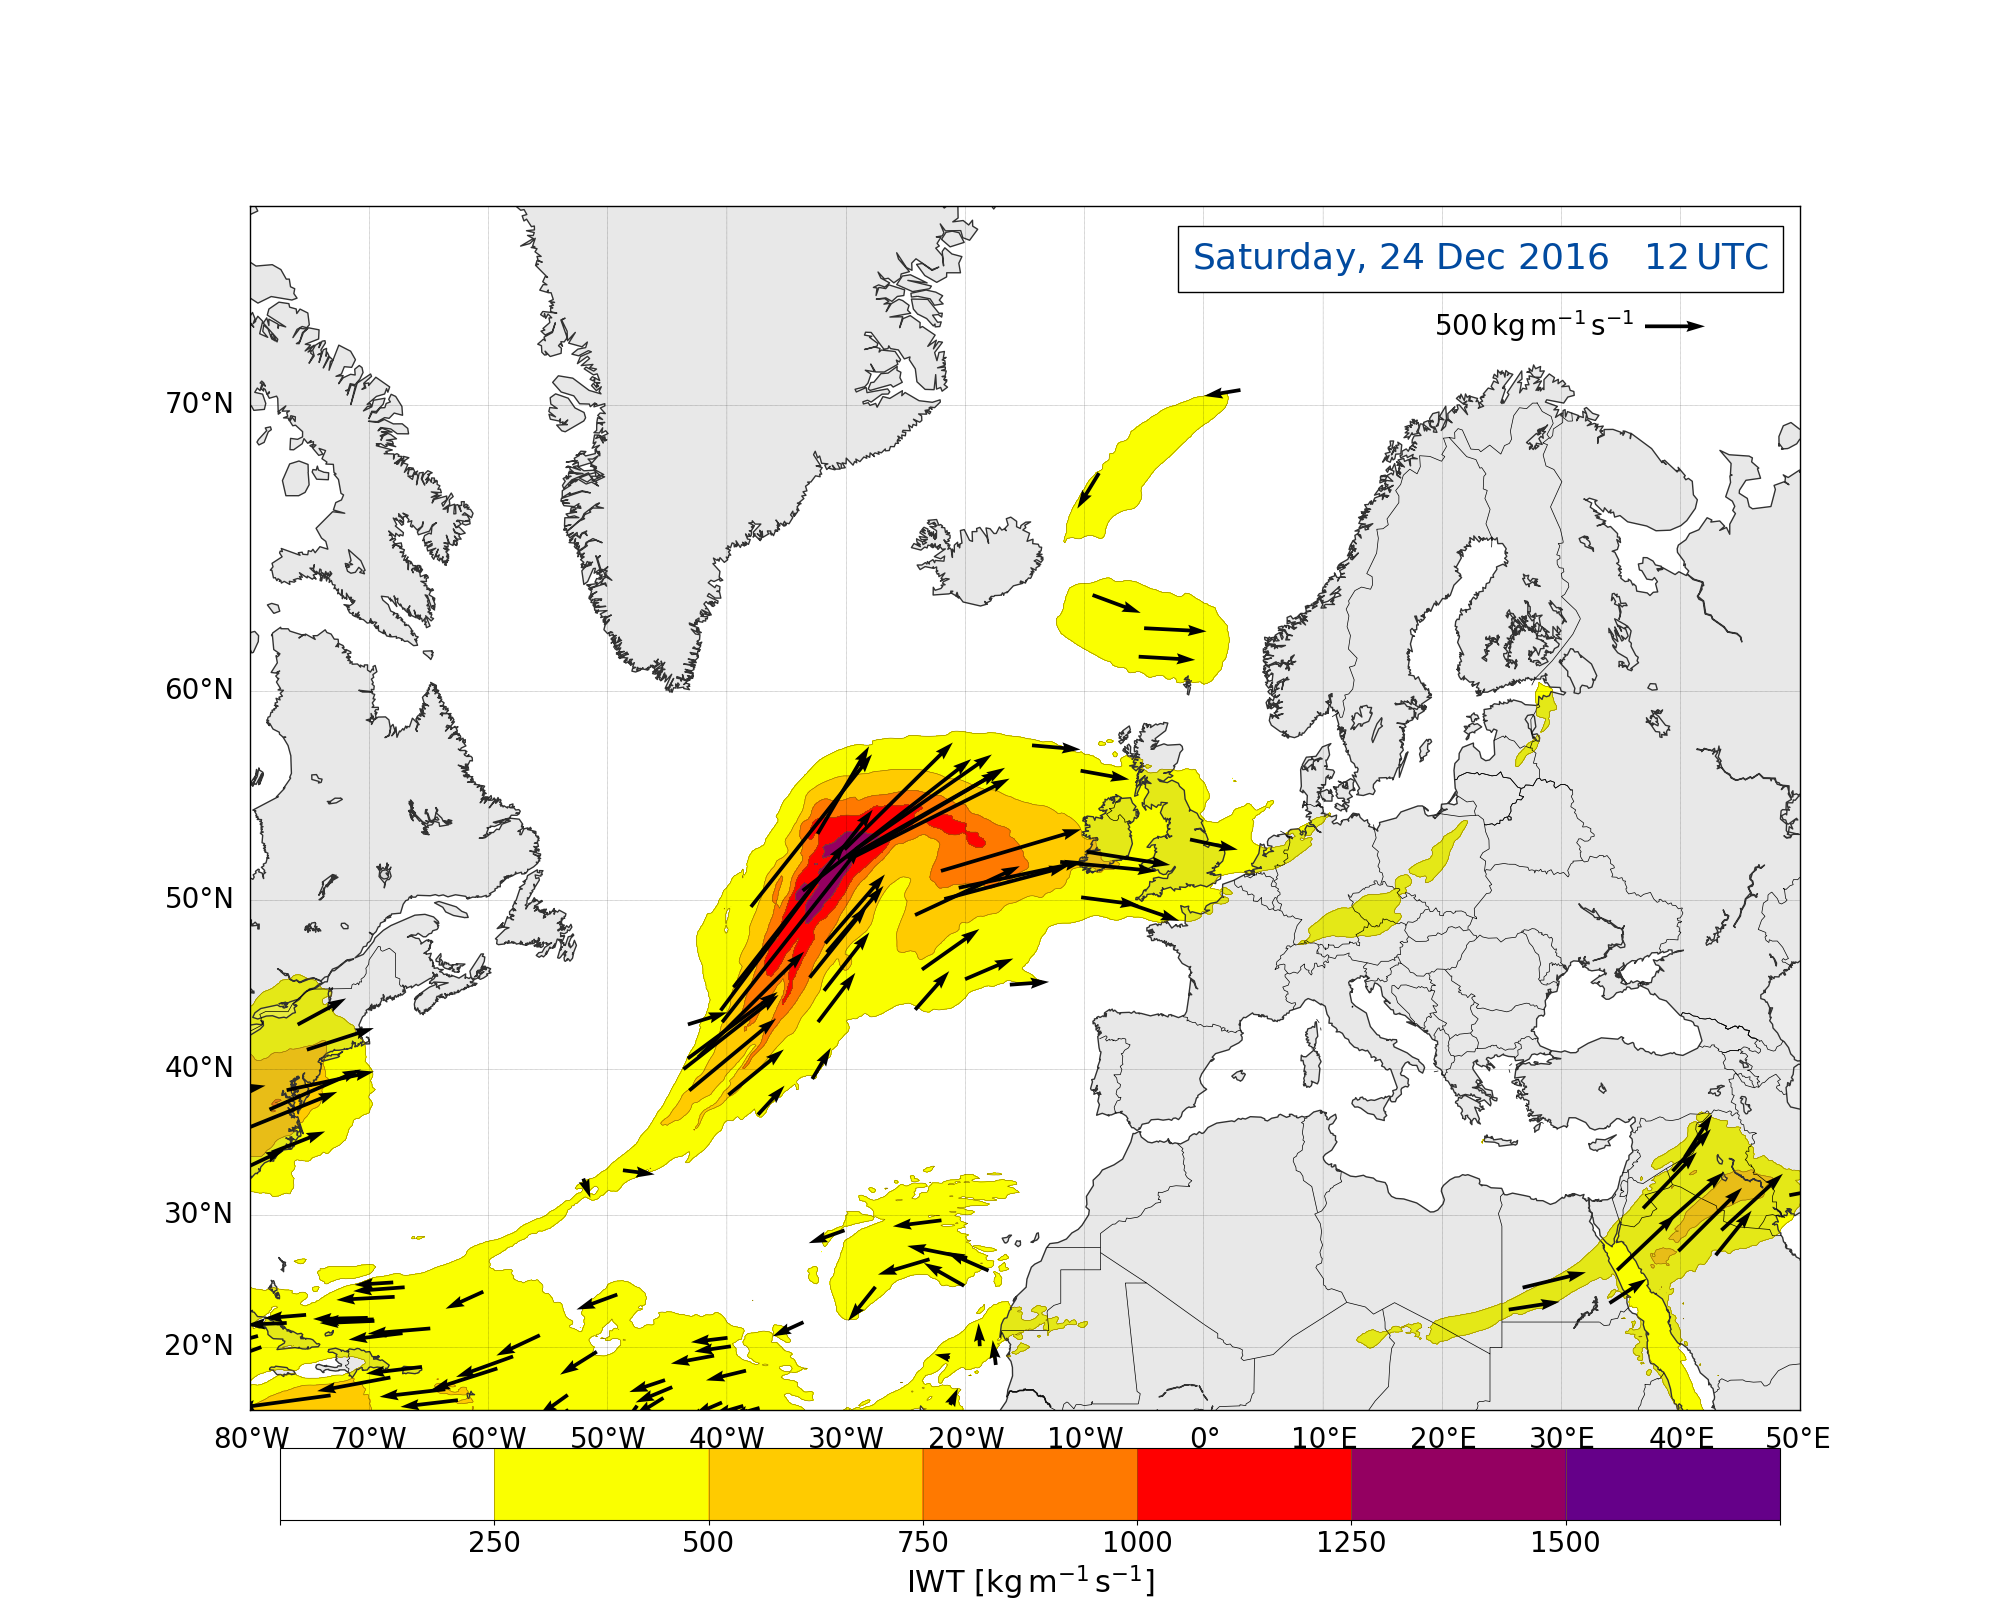
\includegraphics[trim={4.2cm 3.9cm 4.3cm 5.1cm},clip,
		width=\textwidth]{./fig_Atm_Riv/20161224_12}
		\caption{}\label{fig:AR24}
	\end{subfigure}
	%%%%%% 25/12
	\begin{subfigure}[b]{0.49\textwidth}
		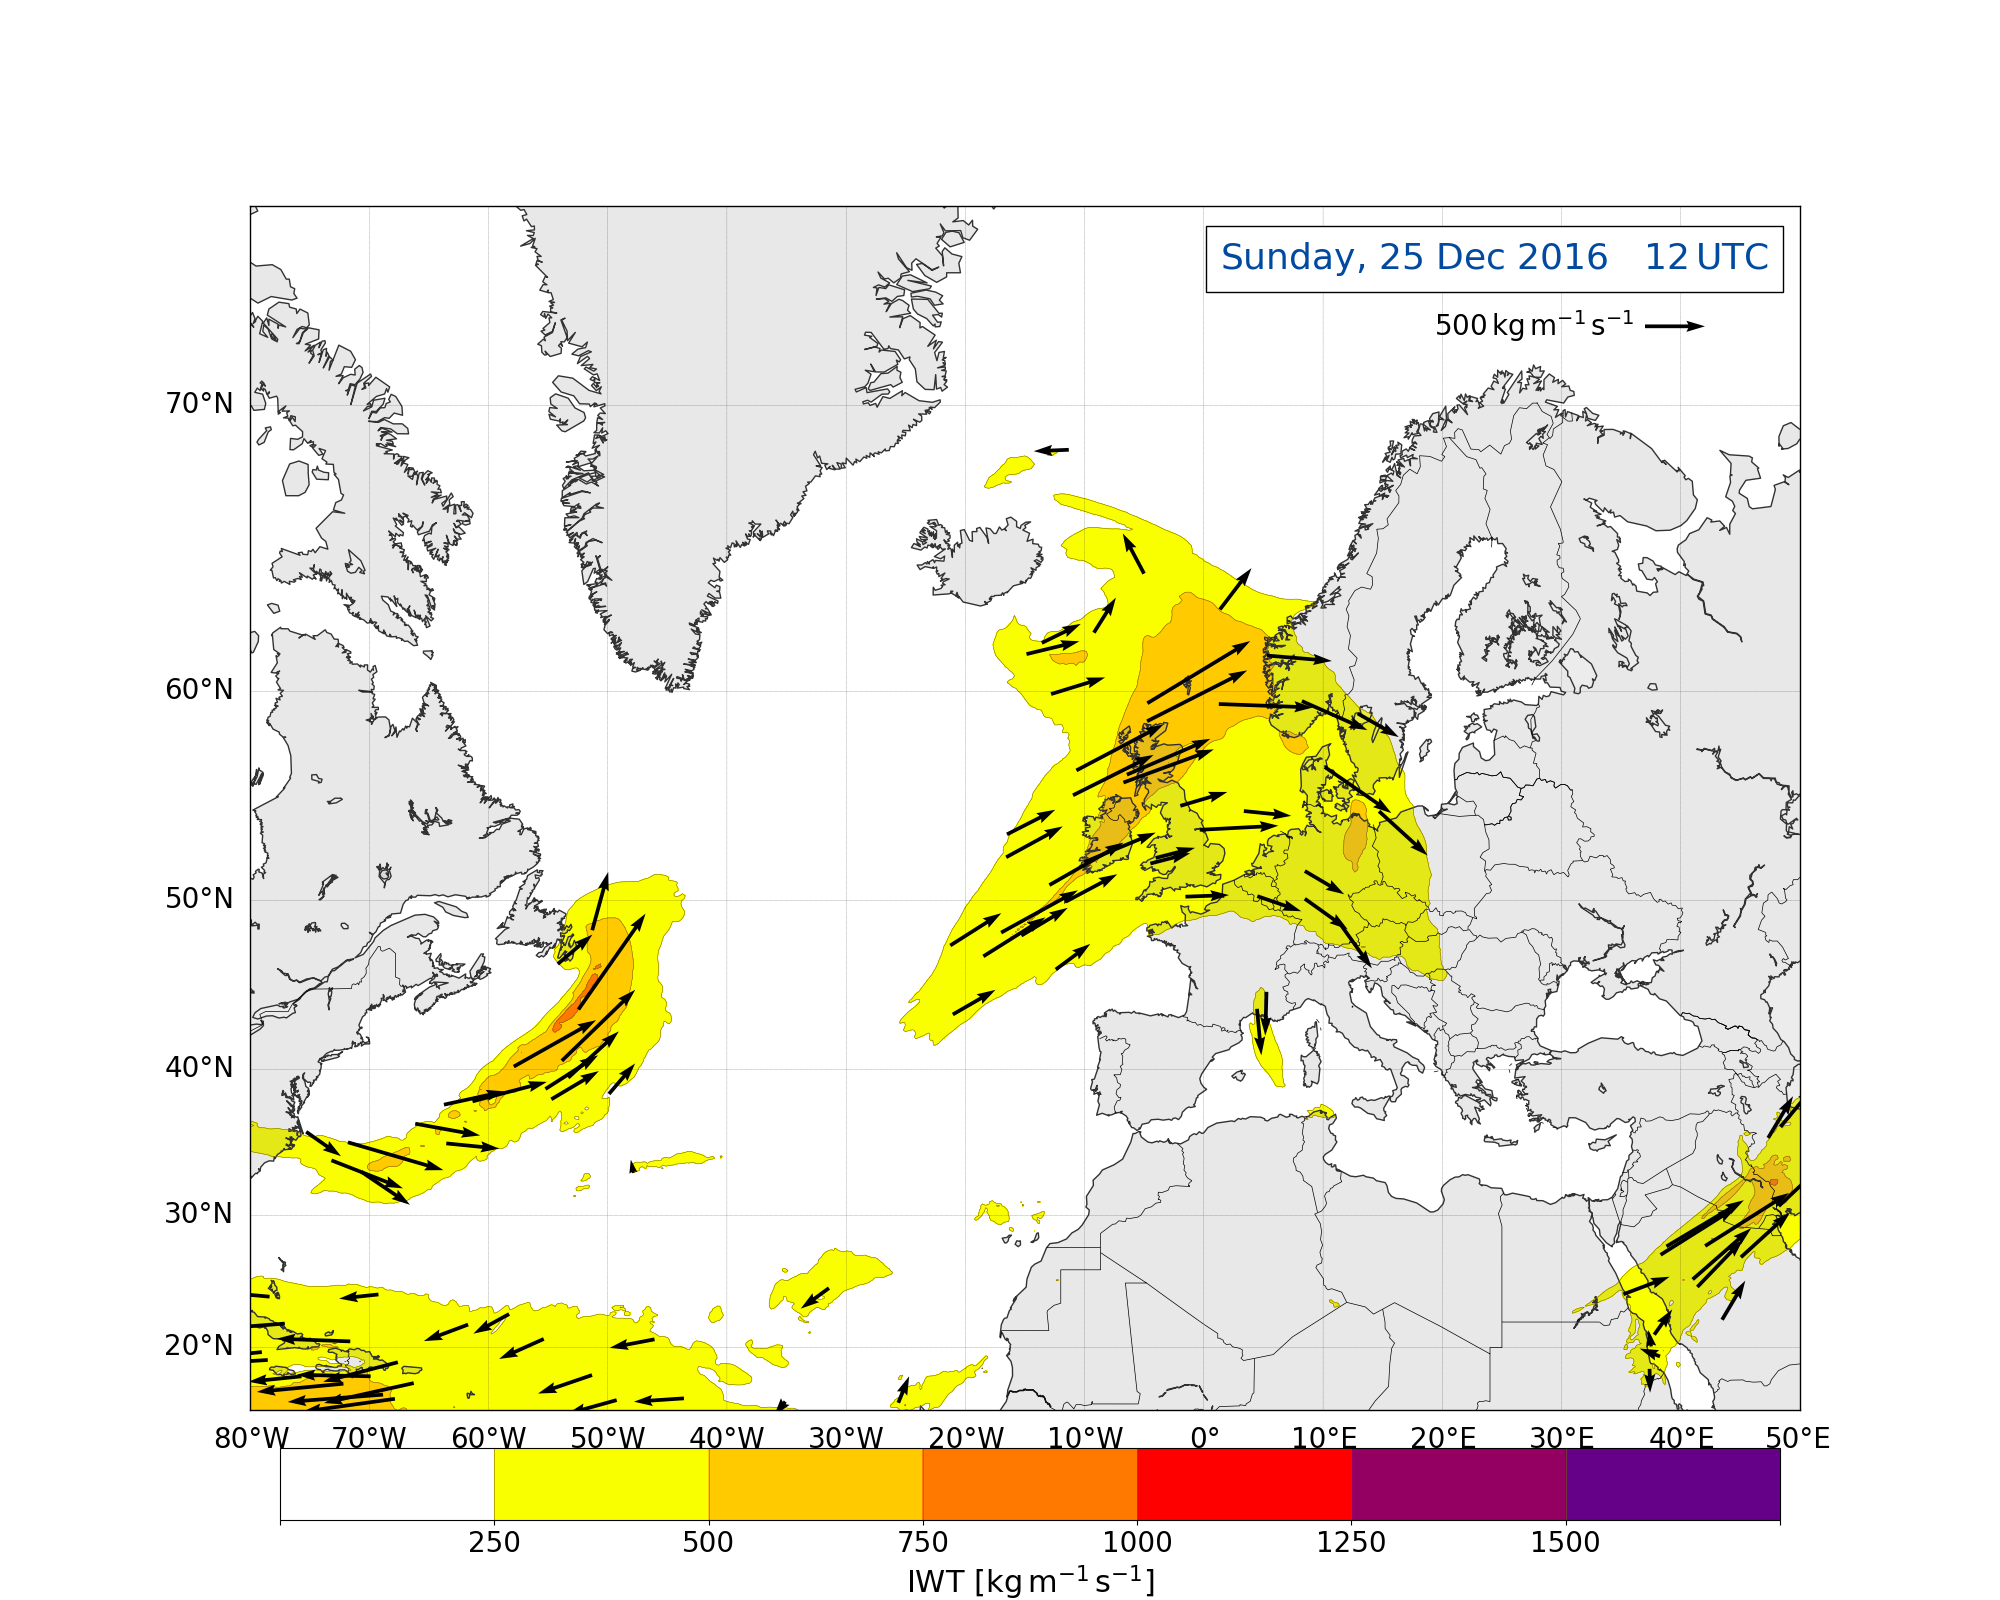
\includegraphics[trim={4.2cm 3.9cm 4.3cm 5.1cm},clip,
		width=\textwidth]{./fig_Atm_Riv/20161225_12}
		\caption{}\label{fig:AR25}
	\end{subfigure}
	%	\centering
	%%%%%% 26/12
	\begin{subfigure}[b]{0.49\textwidth}
		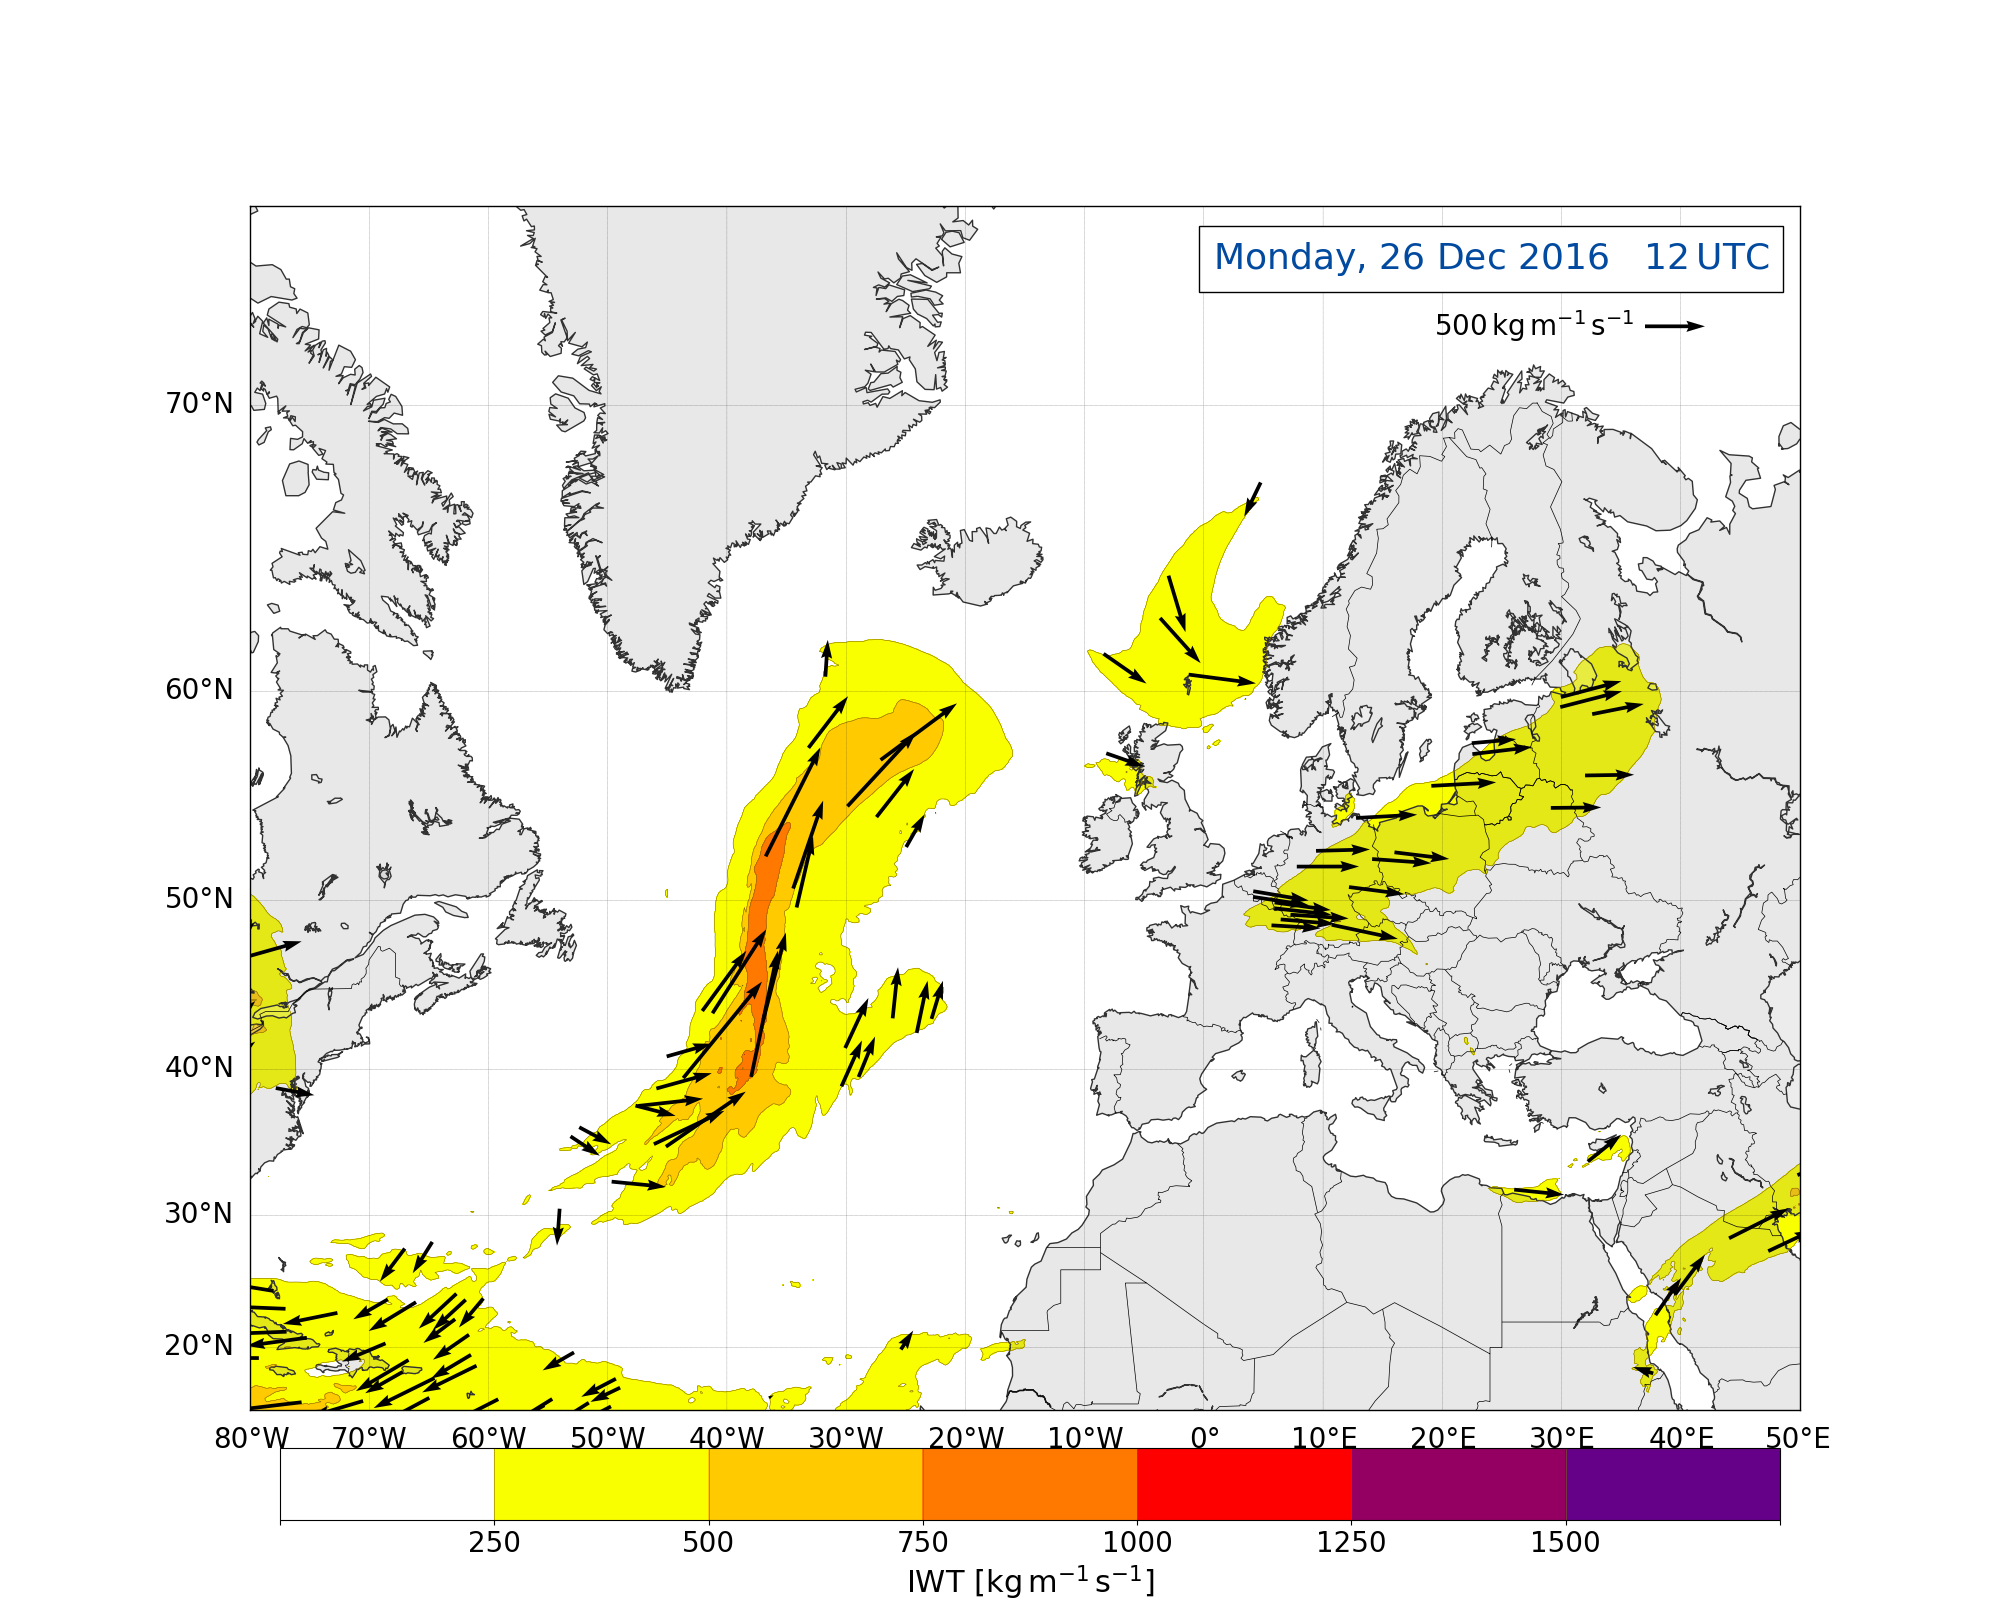
\includegraphics[trim={4.2cm 3.9cm 4.3cm 5.1cm},clip,
		width=\textwidth]{./fig_Atm_Riv/20161226_12}
		\caption{}\label{fig:AR26}
	\end{subfigure}
	%%%%%% 27/12
	\begin{subfigure}[b]{0.49\textwidth}
		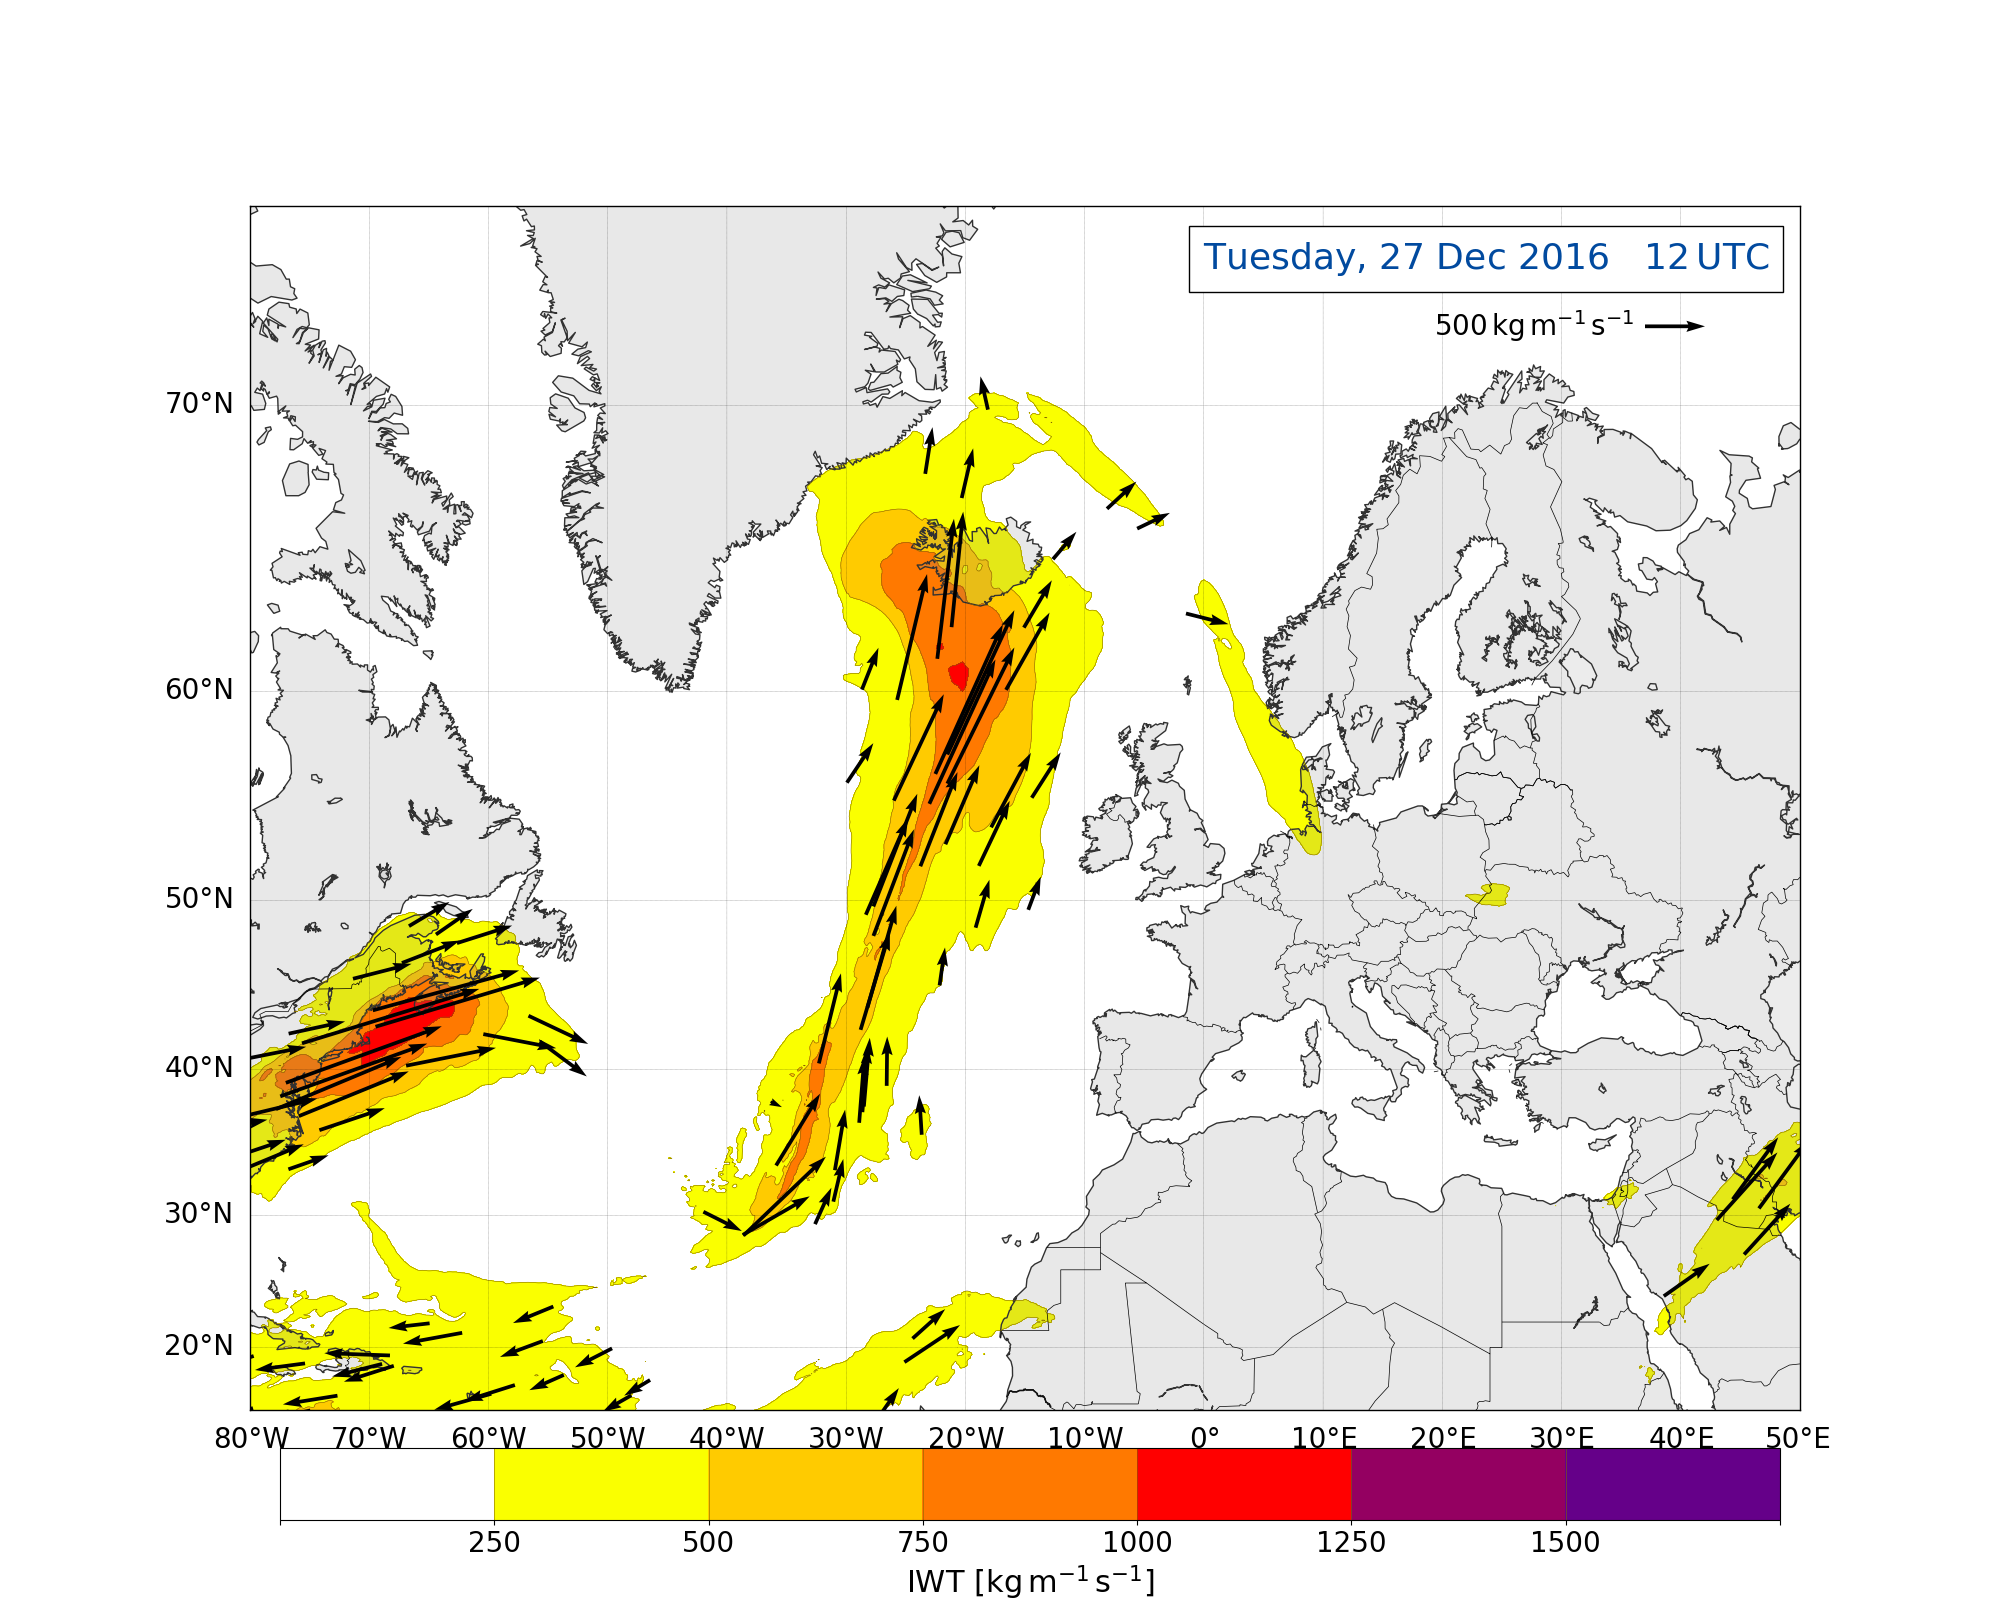
\includegraphics[trim={4.2cm 3.9cm 4.3cm 5.1cm},clip,
		width=\textwidth]{./fig_Atm_Riv/20161227_12}
		\caption{}\label{fig:AR27}
	\end{subfigure}
	%%%%%% label
	\begin{subfigure}[b]{\textwidth}
		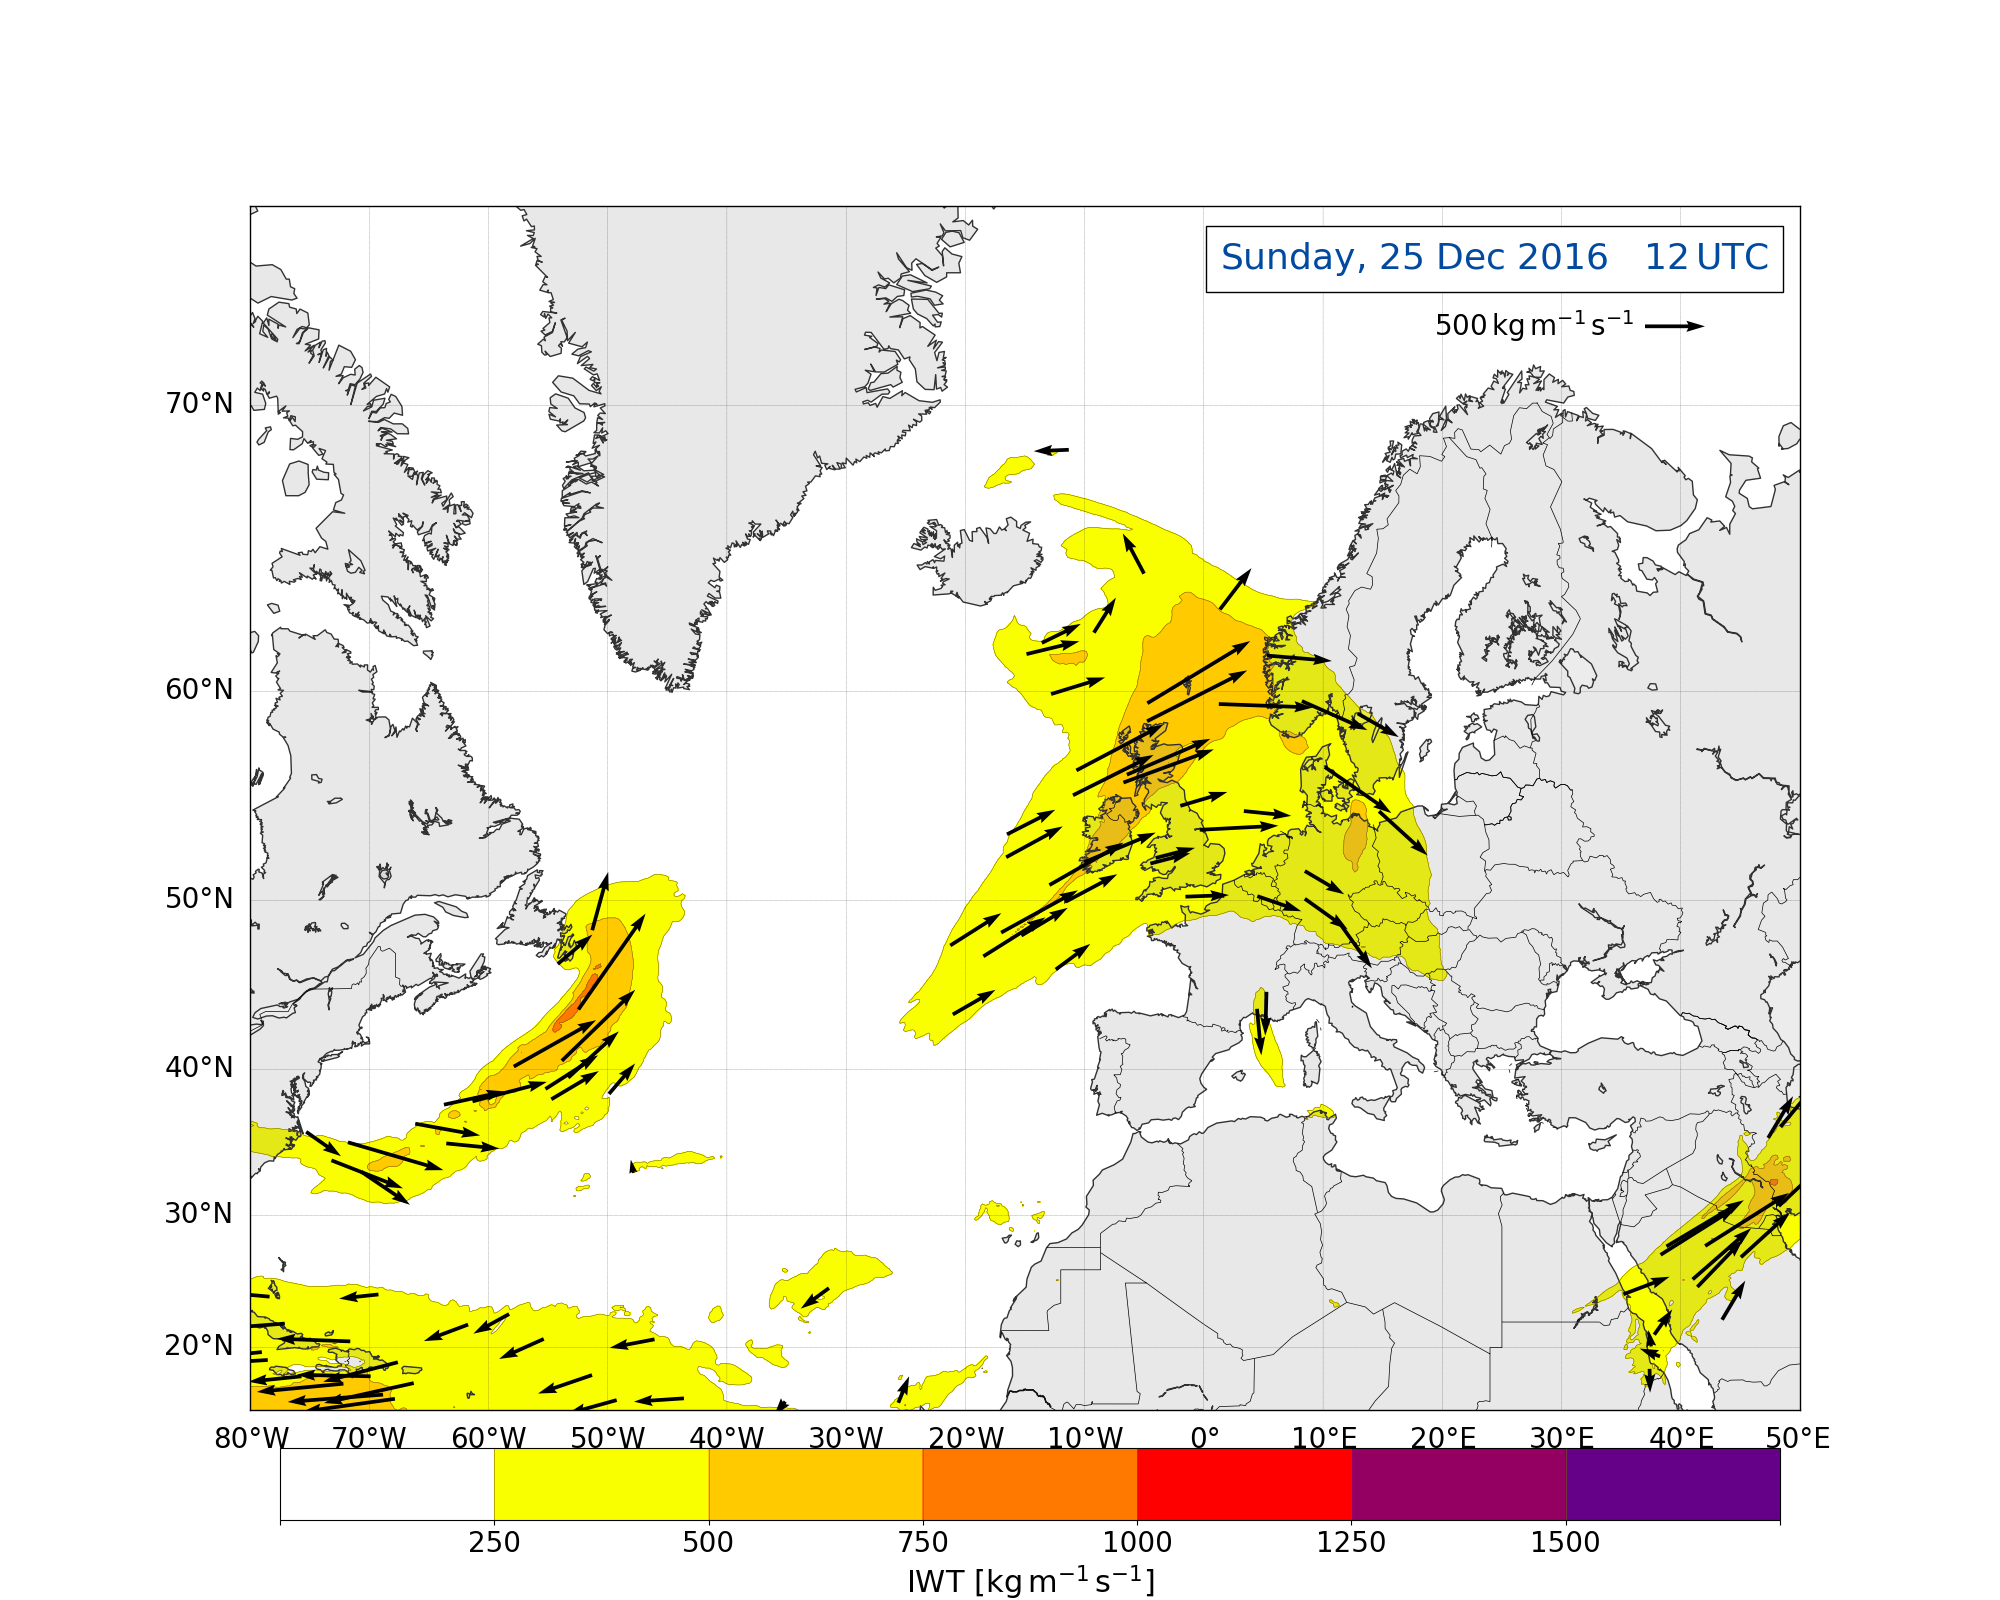
\includegraphics[trim={4.2cm 0cm 4.3cm 36.8cm},clip,
		width=\textwidth]{./fig_Atm_Riv/20161225_12}
	\end{subfigure}
    \caption{\textit{(Continued from previous page.)}}
\end{figure}